\subsection{Gyroskop}
Et gyroskop er et elektromekanisk apparat, som anvendes til at måle vinkelændringer om en given akse, hvilket illustreres på \figref{fig:gyro}. 
\begin{figure}[H]
	\centering
	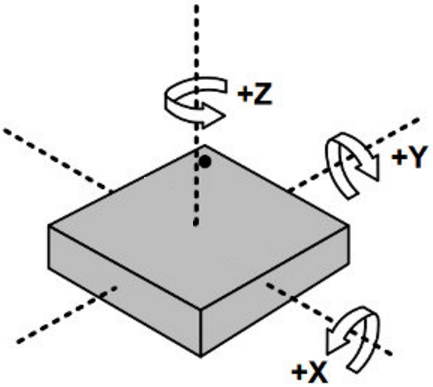
\includegraphics[scale=0.4]{figures/bProblemloesning/gyro.png}
	\caption{På figuren ses et gyroskops måling af rotation omkring x-, y- og z-aksen.~\citep{Sparkfun_gyro} (Modificeret)}
	\label{fig:gyro}
\end{figure}\vspace{-.25cm}
Et gyroskop bestemmer vinkelændringen for en pågældende akse, hvormed enheden for outputtet er grader per sekund (dps). Et gyroskop kan give information om orienteringen eller navigationen af objektet, som sensoren optager data fra. Hvis et gyroskop eksempelvis drejes én omgang om egen akse i sekundet registreres en vinkelændring på 360~dps.~\citep{Sparkfun_gyro,Barbour2014} \newline
Et gyroskop kan eksempelvis registrere vinkelhastighed ved at anvende tyngdekræften og en roterende indre masse~\citep{Sparkfun_gyro,Barbour2014}. Gyroskoper benytter eksempelvis et objekts kræfter ved en cirkulær bevægelse til at bestemme vinkelændringen for det pågældende objekt. Denne type gyroskop kaldes et roterende-masse gyroskop. Et sådant gyroskop benytter kræfterne, som opstår på gyroskopets sensor, når en rotation om en given akse forekommer. Når et gyroskop opsamler data ved cykling mens placeret på benet, vil massen blive udsat for en roterende bevægelse omkring én akse. Massen bliver derved henholdsvis tungere og lettere i processen på baggrund af de ydre påvirkende kræfter, hvorfor outputtet vil komme til udtryk som et sinussignal, hvis det plottes i forhold til tid. Outputtet er afhængig af tyngdekraftens påvirkning af massen, hvorfor et varierende output kræver en bevægelse.~\citep{TittertonWeston2004,Barbour2014,LuingeVeltink2005}

\subsection{Vurdering af accelerometer og gyroskop med henblik på anvendelse}\label{acc_og_gyro}
Et accelerometer kan bestemme den g-påvirkning, som et objekt udsættes for ved en given kraftpåvirkning, hvormed accelerometers ouput angives i g. Derimod bestemmer et gyroskop vinkelændringerne, som et objekt udsættes for, hvoraf gyroskopers output angives i dps. Et gyroskop er, modsat et accelerometer, ikke særligt påvirkeligt overfor støj og vibrationer.~\citep{Goodrich2013,TittertonWeston2004,LuingeVeltink2005} Ydermere har et gyroskop et større strømforbrug sammenlignet med et accelerometer. Et gyroskop er fordelagtig at benytte til blandt andet detektering af gang, løb og cykling. Gyroskopet har dog et større strømforbrug i forhold til et accelerometer, at den oftest udskiftes med et accelerometer til detektering af gang og løb. Dette fremgår yderligere af en række studier, som alle benytter accelerometer til detektering af gang og løb.~\citep{Sparkfun,Rueterbories2010,ClelandKikhia2013} \newline
Som beskrevet i \secref{bevaegelse} er der en stor påvirkning af et accelerometer i y-aksens retning ved gang og løb. Et accelerometer er derfor fordelagtigt at benytte til detektering af disse aktivitetsformer for at reducere strømforbruget af et eventuelt system. Dette er grundet sensorens lave strømforbrug, samt accelerometerets egenskab til at detektere gang og løbs karakteristika. Derimod er et gyroskop fordelagtigt at benytte til detektering af cykling, idet denne bevægelse er en cirkulær bevægelse omkring en akse. Betydningen heraf vil medføre, at cykling tilnærmelsesvis kan afspejles som en sinussignal med varierende frekvens og amplitude afhængigt af hastigheden.~\citep{TittertonWeston2004,LuingeVeltink2005} \newline
Dette projekt vil derfor benytte et accelerometer til detektering af gang og løb samt et gyroskop til detektering af cykling.